\section{MITM attack and honeypots}
%Does a honeypot could help in the protection from the MITM attack?
%First we need to explain what is a MITM attack. 
In a server-client architecture, a MITM attack takes place when the attacker is inserted inside the communication between client and server. Let's make an example of possible situation that could occur, and a proposal of honeypot that could resolve it. \\
The normal procedure to avoid MITM attack is to encrypt and decrypt data between client and server. The main steps are:
\begin{enumerate}
    \item \textbf{Use asymmetrical encryption}. First we use an asymmetric algorithm to allow us to send in a secure way the symmetric key that will be used in the future;
    \item \textbf{Use symmetric encryption}. Now that the symmetric key is shard between the server and the client, the data are sent normally between the ends points and not anyone in the middle can understand them.  
\end{enumerate}

\noindent What if the first step fails? As an example,our IoT server for example could use a weak RSA algorithm, based on 16 bit key. Our men in the middle could manage to find the private key of the server and decrypt the symmetric key that will be used in the second step, like shown in the figure below.

\begin{figure}[h!]
  \centering
  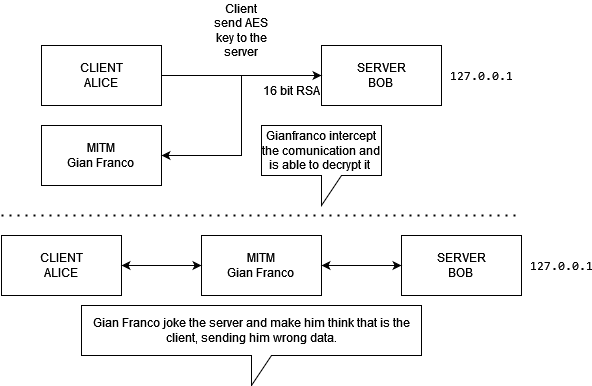
\includegraphics[width = 15cm]{images/MITMExampleAttack.drawio.png}
  \caption{An example on MITM attack}
  \label{fig:4period}
\end{figure}
\FloatBarrier

\noindent How can our system understand that it is speaking to a MITM and not to the client? Our honeypot would intervene right here.\\
For example, it could first check if the wrong data sent by the MITM makes sense or not. Then it could check if the data of the fake sensor makes sense with respect to a set of data collected from the real sensor in the precedent days. If the honeypot recognizes that a man in the middle is present, it could collect data about the hacker and see what information they are trying to capture, which attacks he/she is trying to inject in to the network, studying  the methodology used by hackers. Moreover, a honeypot AP could (at least temporarily) keep the hacker engaged and alert the administrator so that the actual network can be safeguarded.then close the collection. If no violation is detected, the honeypot sends the data to the real server. A possible implementation is show in the figure below.

\begin{figure}[h!]
  \centering
  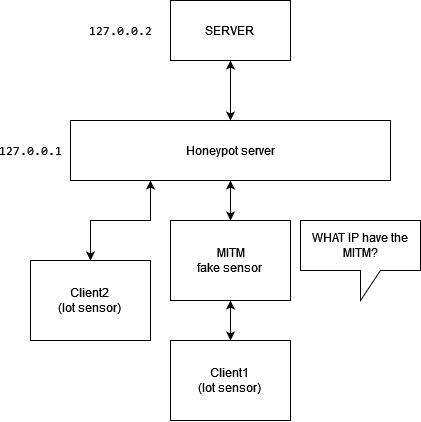
\includegraphics[width = 15cm]{images/MITMHONEYPOT.drawio.png}
  \caption{A possible system structure for the MITM honeypot.}
  \label{fig:5period}
\end{figure}
\FloatBarrier

\section{FAKEHONEYMITM (MITM attacks and honeypots)}
Regarding the MITM attack, we have another possible idea to implement. As we know, a man in the middle tries to place himself between the sensors of the IoT cluster and the servers inside the network. He need to intercept the message from the sensors to the servers and viceversa. But what if the sensor is not real but is a honeypot? For example our cluster could expose a connection between 2 honeypots, the first one is a fake server, the second one is a fake sensor. But why an attacker have to choose this connection for him malicious purpose? Well, this link could work with a weak encryption to seems like a vulnerability of our network. When the MITM manage to put itself between the fake connection, our honeypots could collect data on the activity of the hacker. To better understand this idea, please refer to the figure (\textcolor{blue}{\ref{fig:MITMFakeSensor}})

\begin{figure}[h!]
  \centering
  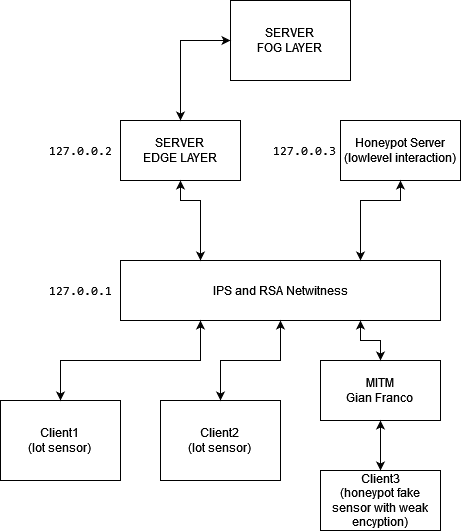
\includegraphics[width = 10cm]{images/MITMFakeSensor.drawio.png}
  \caption{A possible structure for the fake sensor honeypot and MITM}
  \label{fig:MITMFakeSensor}
\end{figure}
\FloatBarrier


